\documentclass[../main.tex]{subfiles}
\graphicspath{{\subfix{..}}}

\begin{document}
\chapter{Reliability of machine learning methods}
\label{sec:janne}

\epigraph{``Psychohistory was the quintessence of sociology; it was the science of human behavior reduced to mathematical equations. The individual human being is unpredictable, but the reactions of human mobs, Seldon found, could be treated statistically''}{Isaac Asimov, Second Foundation}

\minitoc

As explained in previous chapters, JUNO is a precision experiment where the complete understanding of the effects at hand is crucial. As it will be illustrated in Chapter \ref{sec:joint_fit}, even small invisible biases or uncertainties could lead to the imposibility to run the measurements, or even worse, wrong our mass ordering measurements. While the liquid scintillator technology is well none and straightforward, this is the first time it is deployed to such scale, and for such precision. This novelty bring its fair share of elements, effects or assumption, that, if they were to be overlooked, could cause issue.

We already shown a large variety of reconstruction algorithms, OMILREC for LPMT reconstruction in Section \ref{sec:juno:reco}, numerous machine learning algorithms in section \ref{sec:juno:ml} and our own work in chapters \ref{sec:jcnn} and \ref{sec:jgnn}. Those algorithms were compared to each others based on their performance as in \cite{qian_vertex_2021} but we are the first that looked into the correlation between the reconstruction. The combinations of algorithms shown in Chapter \ref{sec:jcnn} show that some information elude the algorithms. We used this fact to try to improve our performance but this could also lead the algorithm to being vulnerable to some effect that could affect the detector and wrong the measurements.

The search for such effect could be done by hand, but the process would be tedious. We propose in this thesis a machine learning method to probe for those effects.  In Section \ref{sec:janne:method}, I describe the method behind the algorithm. In section \ref{sec:janne:arch} I detail the architecture of our algorithm and in section \ref{sec:janne:results} the results of it. Finally, in section \ref{sec:janne:conclusion}, I conclude and discuss about the prospect and possible improvements to bring to this work.

\section{Method}
\label{sec:janne:method}
%\begin{itemize}
%  \item JUNO needs very good understanding of reconstruction
%  \item Estimator combination shows that there can be improvement due to simplfication and that NN/reco methods can have hard time grasping all the detector effect.
%  \item If there is potential failure point, we need to search for them
%  \item La mesure de la NMO est tres sensible (see $alpha_{qnl}$ joint fit chapter)
%\end{itemize}

As introduced above, JUNO needs a very good understanding of the biases and effects affecting its reconstruction as a small bias could wrong the mass ordering measurement. To calibrate those biases and effect, JUNO rely on multiples sources that can be located at various point in the detector. The calibration strategy was already discussed in Section \ref{sec:juno:calib} and show calibrations sources of gammas, neutrons and positrons, with the catch that the positrons will annihilate inside the encapsulation and only the two 511 keV gammas will be seen.

None of the calibrations sources considered are positron event. While electrons and positrons events should be pretty similar in their interaction with the electronic cloud of the LS atoms, electron events are missing the two annihilations $\gamma$ and the potential of forming a positronium \cite{schwarz_measurements_2018}. The topology of the event thus differ of the order of magnitude of our reconstruction performance. A few nanoseconds between the energy deposit and  the positronium annihilation against a time transit spread between 3 and 6 ns depending on the PMT type \cite{rodphai_20-inch_2021, liao_study_2017, li_characterization_2018}. The $\gamma$ from the positron annihilation will travel distances of the order of magnitude of the typical LPMT resolution of 8 cm (see Section \ref{sec:juno:reco}).

Another natural calibration source is the $^{12}B$ spectrum. The $^{12}B$ is a cosmogenically produced isotope through the passage of muons inside the LS. The $^{12}B$ decays via $\beta^-$ emissions with a Q value of 13.5 MeV with more than 98\% of the decay resulting in ground state $^{12}C$. The $^{12}B$ event will be cleanly identified by looking for delayed high energy $\beta$ events after an energetic muon. Due to its natural causes, the $^{12}B$ events will be uniformly distributed in the detector. The calibration strategy consist in fitting the energy spectrum of $^{12}B$ with the results of the simulation to adjust the simulation parameters. Both sources will be used to \textit{control} the response of the detector.

Unlike lasers and radioactive, from which the localization and energy will be well known, the individual truth of $^{12}B$ will be unknown with only the localisation loosely constrained by the muon track. Only higher order observables such as the energy distribution will be accessible.

All of those considerations could hide potential unknown or undetected effect that could lead to issue in the mass ordering analysis. But, while we have idea from where the issue could come, the production by hand of event perturbations that go unseen in the calibration would be tedious. That's why we propose to use an Adversarial Neural Network (ANN) to produce those perturbations if they exists. A schematic of the concept is presented in Figure \ref{fig:janne:method:schema}.

\begin{figure}[ht]
  \centering
  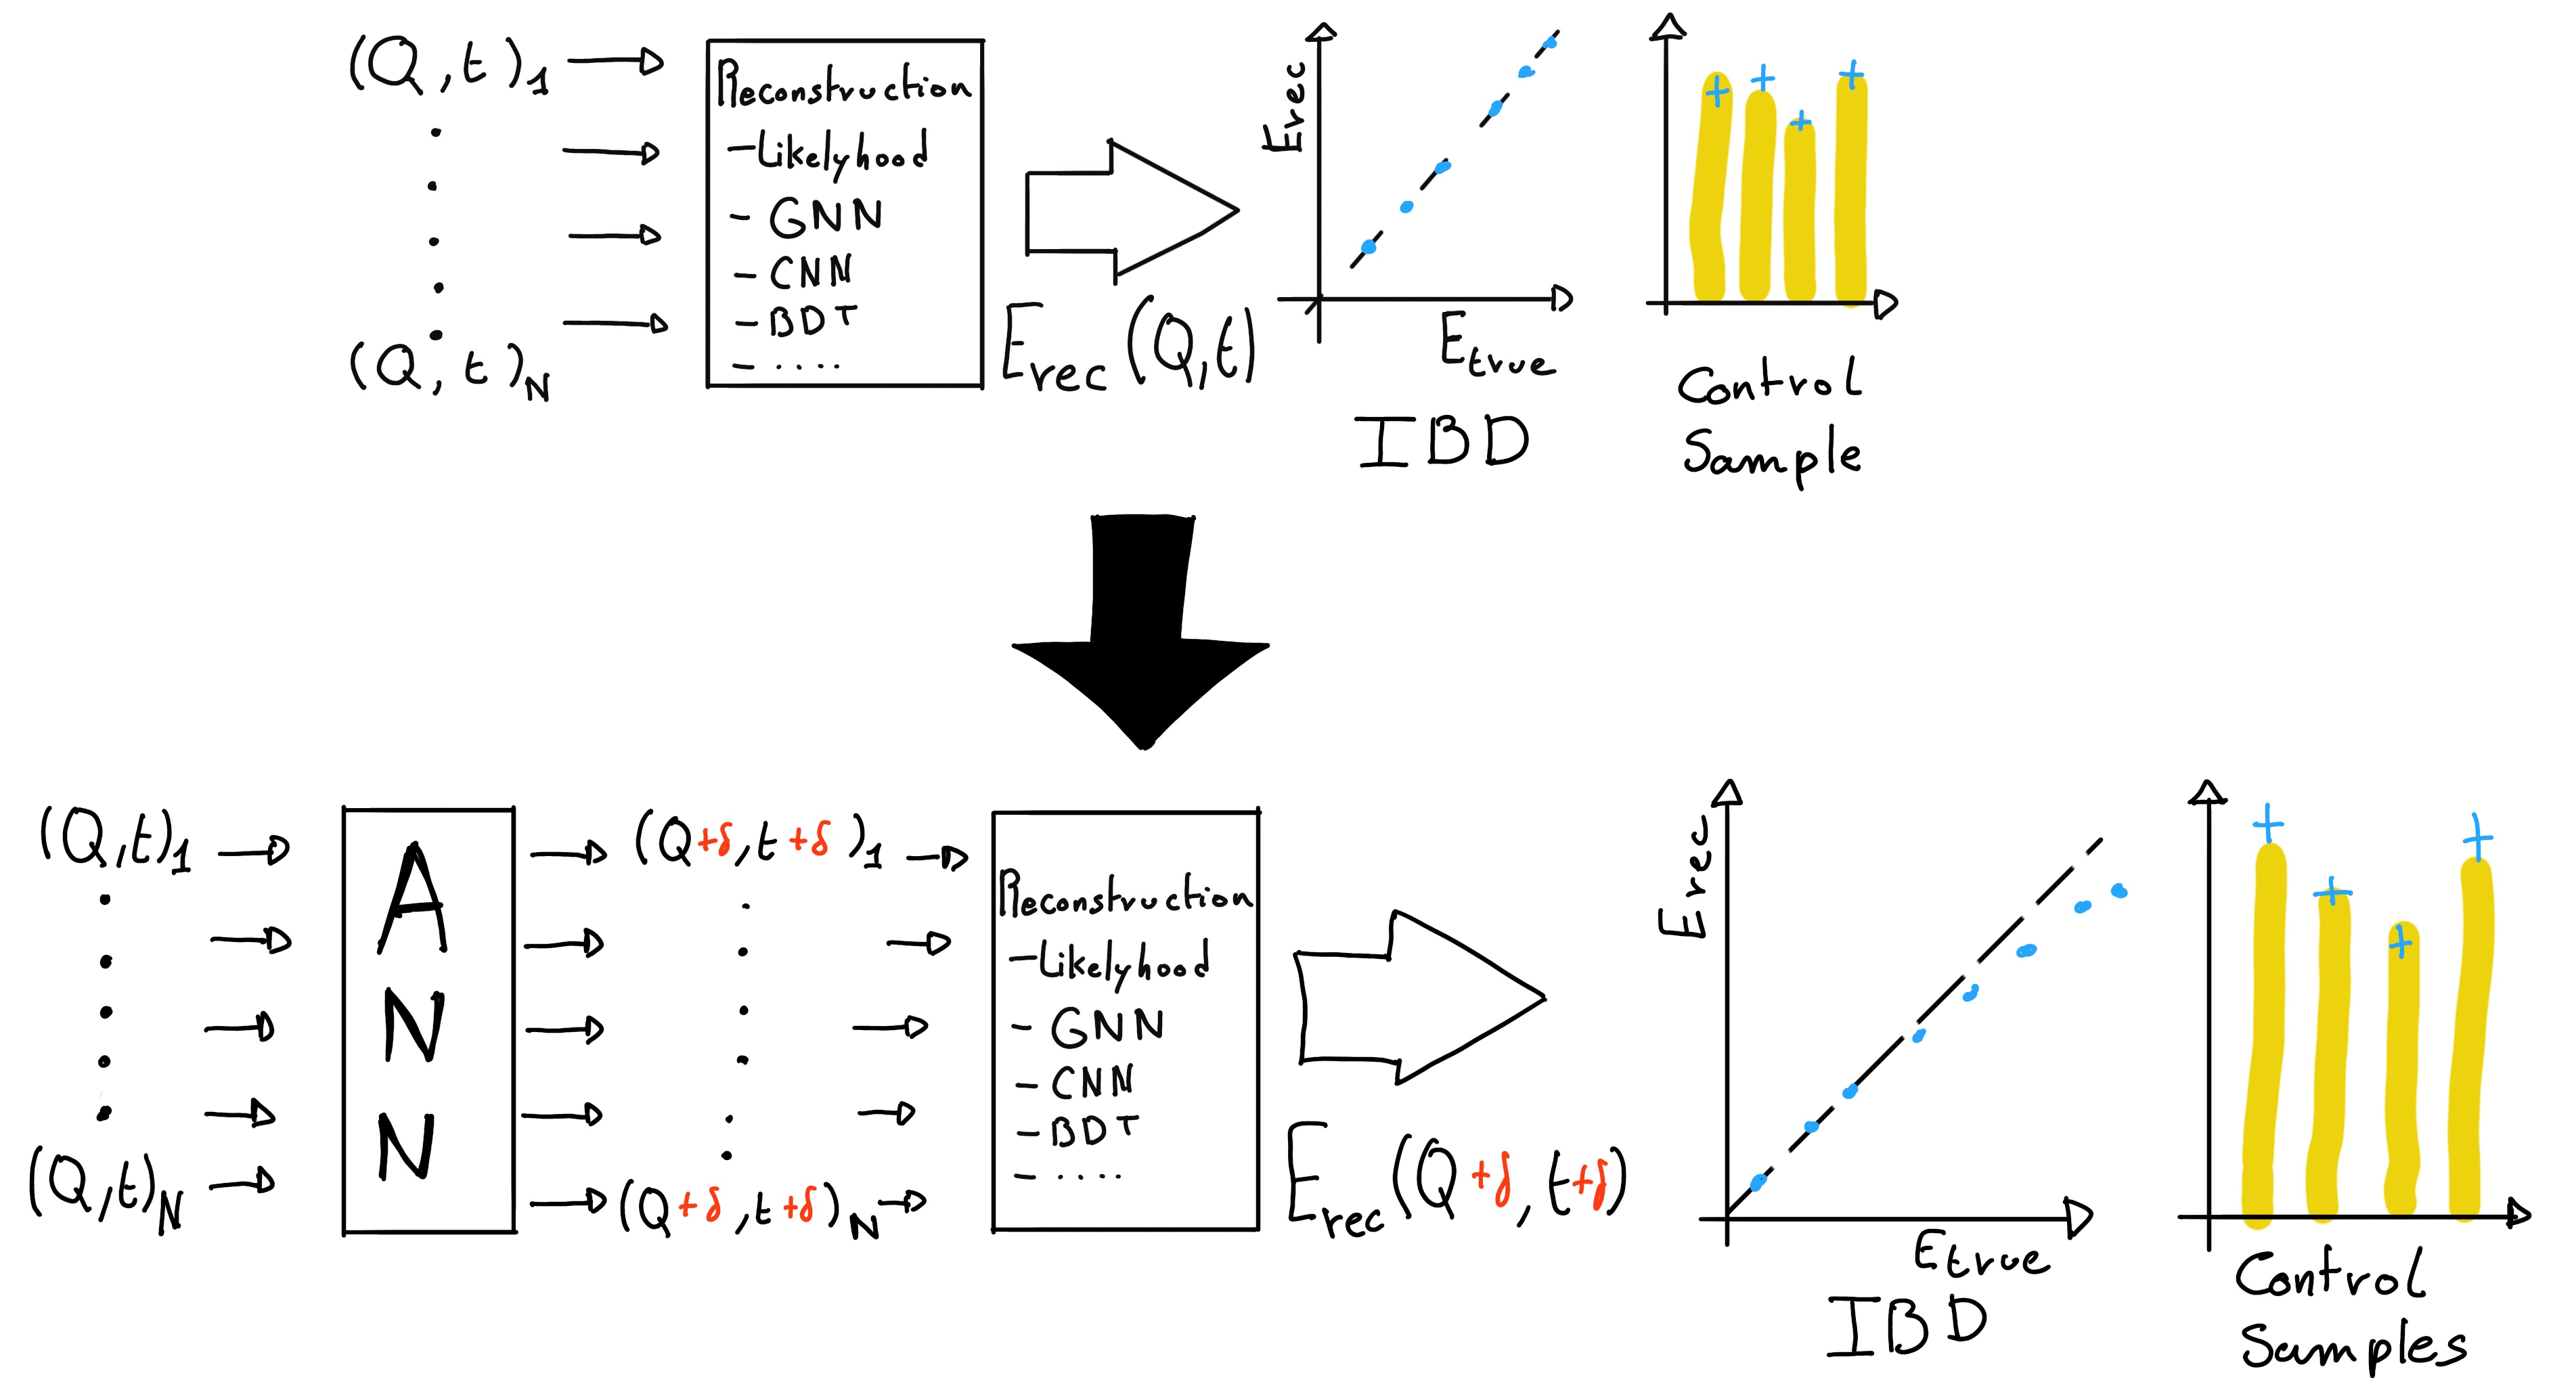
\includegraphics[width=\linewidth]{images/janne/ann_method.jpg}
  \caption{Schema of the method to discover vulnerabilities in the reconstruction methods. \textbf{On the top} of the image, the standard data flow. The individual charge and times are fed to a reconstruction algorithm. From the reconstructed energies, we can produce an IBD spectrum and compute control observables from the control samples. \textbf{On the bottom}, the same data flow but we add an ANN between the input and the reconstruction. The ANN will slightly change the input charge and time so the reconstruction algorithm inaccurately reconstruct the IBD energy, but the perturbation is not visible in the control sample.}
  \label{fig:janne:method:schema}
\end{figure}

This network should produce physically sound perturbation, that would not be seen by the calibration but also by the visualisation of the event. If the ANN manage to produce such perturbations, we can derive systemic uncertainties from it. If it fail to find some, it is a proof of robustness for the attacked reconstruction method.

For this study we consider a ``physics'' dataset composed of 1M positron events from J23, uniformly distributed in the Central Detector (CD) and in deposited energy between $E_{dep} \in [1.022; 10.022]$. This set represent the IBD events we want to \textit{wrongly} reconstruct.

We use a second ``control'' dataset of electron event also uniformly distributed in the detector and over the same energy range. They mimic the energy deposit of $^{12}B$ decay and are used as the sample to compute the control observables.

\section{Architecture}
\label{sec:janne:arch}
%\begin{itemize}
%  \item Expliquer la problematique dans l'architecture
%  \item Ambition de pouvoir etre appliqué a toutes les methodes, pas que NN
%  \item Pb techique: descente de gradient
%  \item Présenter la loss
%\end{itemize}
We can describe the goal of the ANN by the following loss function:
\begin{equation}
  \label{eq:janne:loss}
  \mathcal{L} = \mathcal{L}_{adv} + \mathcal{L}_{reg}
\end{equation}
where $\mathcal{L}_{adv}$ is the adversarial loss, which is minimal when the reconstruction is ``broken''. We thus need to define what is a \textit{wrong} reconstruction. We choose to define it via the correlation between the reconstructed and deposited energy
\begin{equation}
  \label{eq:janne:ladv}
  \mathcal{L}_{adv} = |\mathrm{Corr}(E'_{rec}, E_{rec})|
\end{equation}
where $E'_{rec}$ and $E_{rec}$ are the reconstructed energies after and before perturbation respectively.
This loss is positive or null and is minimal when the reconstructed energy after perturbation is decorrelated with the original reconstruction.

The term $\mathcal{L}_{reg}$ is the regularisation term, which is minimal when the control variable are correctly reconstructed
\begin{equation}
  \mathcal{L}_{reg} = \sum_\lambda (O^{rec}_\lambda - O^{th}_\lambda)^2
\end{equation}
where $\lambda$ index the different control observables that will be considered in this study. It's minimal when the control observables after perturbation $O^{rec}_\lambda$ are coherent with their expected values $O^{th}_\lambda$.
In this exploratory work, we choose as the control observable the difference between the reconstructed position and energy and the ground truth from the Monte Carlo simulation complemented with a penalty term $P$
\begin{equation}
  \label{eq:janne:lreg}
  \mathcal{L}_{reg} = \sum_{\lambda \in \{x, y, z, E\}} (\lambda_{rec} - \lambda_{true})^2 + P
\end{equation}
This penalty $P$ is here to prevent the ANN from producing event too different from the initial event. It will be further detailed in Section \ref{sec:janne:arch:ann}
.

We see that the final loss is the equilibrium between the adversarial and regularisation loss.

\subsection{Back-propagation problematic}
\label{sec:janne:back_prop}

We would like this method to be applicable to any kind of reconstruction algorithm but this complicated considering standard training method through backward-propagation, discussed in details in Section \ref{sec:ml:optim}. For explanation, let's define the application of the reconstruction algorithm as $\mathcal{F}$ on an event $X$, resulting in the prediction $Y$ and the application of the ANN $\mathcal{G}$ on $X$ to give a perturbed event $X'$, we can parametrize the equation \ref{eq:janne:loss}
\begin{align}
  Y = \mathcal{F}(X); ~~& Y' = \mathcal{F}(X') = \mathcal{F}(\mathcal{G}(X))
\end{align}
\begin{equation}
  \mathcal{L} \equiv \mathcal{L}(\mathcal{F}(\mathcal{G}(X)), Y_t)
\end{equation}
where $Y_t$ is the reconstruction target of $Y$.

Now if we consider a parameter $\bm{\theta}$ of the ANN on which we want to optimize $\mathcal{L}$, in the backward-propagation optimisation framework we need to compute
\begin{equation}
  \frac{\partial \mathcal{L}(\mathcal{F}(\mathcal{G}(X)))}{\partial \bm{\theta}}
\end{equation}
which, when using the chain rule, become
\begin{equation}
  \frac{\partial \mathcal{L}(\mathcal{F}(\mathcal{G}(X)))}{\partial \bm{\theta}} = \frac{\partial \mathcal{G}}{\partial \bm{\theta}} \cdot \frac{\partial \mathcal{F}}{\partial \mathcal{G}} \cdot \frac{\partial \mathcal{L}}{\partial \mathcal{F}}
\end{equation}

The terms $\frac{\partial \mathcal{G}}{\partial \bm{\theta}}$ and $\frac{\partial \mathcal{L}}{\partial \mathcal{F}}$ are easily computable but $\frac{\partial \mathcal{F}}{\partial \mathcal{G}}$ depends on the nature of the reconstruction algorithm. While it comes naturally when using NN algorithms, it's not so trivial for other kind of algorithms like likelihood. Solutions exists to optimize networks that work in complex, non differentiable environments, such as \textit{Deep Reinforcement Learning} \cite{kiran_deep_2021, vinyals_grandmaster_2019} but as a first prototype we will restrict ourselves to neural networks for the reconstruction algorithm.

The choice to use gradient descent, and therefore neural network, also allowed us to keep all technical software development wrapped in the same language and framework, PyTorch \cite{ansel_pytorch_2024}.

The backward-propagation introduce a second issue. At the beginning of the subsection we introduce $X' = \mathcal{G}(X)$, the event after perturbation. It's an input of the reconstruction $\mathcal{F}$, thus, let's say that the event, in its form $X$, is a list of tuples $(id, Q, t)$ which are the hit on the PMT $id$. If $\mathcal{F}$ require the information to be formatted in a specific way (graph, images, ...) via an algorithm $\tau(X)$, it means that
\begin{equation}
  \frac{\partial \mathcal{L}(\mathcal{F}(\tau(\mathcal{G}(X))))}{\partial \bm{\theta}} = \frac{\partial \mathcal{G}}{\partial \bm{\theta}} \cdot \frac{\partial \tau}{\partial \mathcal{G}} \cdot \frac{\partial \mathcal{F}}{\partial \tau} \cdot \frac{\partial \mathcal{L}}{\partial \mathcal{F}}
\end{equation}
which also requires that $\frac{\partial \tau}{\partial \mathcal{G}}$ is differentiable.

On the other hand, if $X$ is already formatted as the input of $\mathcal{F}$, it mean that $\mathcal{G}$ take the same format as input and we drop the requirement on $\tau$ to be differentiable. Concretely, if $\mathcal{F}$ takes an image as input, it mean that $\mathcal{G}$ will also takes an image as input and output an image. That also unfortunately mean that if some informations is loss before $\mathcal{G}$, for example during the charge and time aggregation in pixels, it cannot retrieve and modify it.

A more elegant solution would that $\mathcal{G}$ would also compute the transformation $\tau$ in addition to finding relevant perturbation, but for the simplicity of this exploratory work, we use a $\mathcal{G}$ that process transformed data.

\subsection{Reconstruction Network (FFNN)}
\label{sec:janne:arch:reco}
%\begin{itemize}
%  \item Reseau de Neurone Simple. Deux avantages:
%  \item Besoin pour la descente de gradient
%  \item Un reseau "simpliste" a plus de chance de présenter des "défauts" que l'ANN pourrait exploiter
%\end{itemize}

As introduced just before, we need a NN algorithm for IBD reconstruction. We could have used the GNN presented in Chapter \ref{sec:jgnn} but we preferred a more simplistic approach to not be constrained by the memory consumption of the reconstruction neural network. This network is designated as FFNN.

This network takes as input a vector containing the results of the aggregation of charge and time on pixels. We consider JUNO composed of 3072 pixels defined by the Healpix \cite{gorski_healpix_2005} pixelisation. On each of those pixel, we sum the charges and keep the minimal time of hit, resulting in 3072 $(Q, t)$ tuples. To those tuples, we adjoin the position of the center of those pixels, resulting in 3072 $(Q, t, x, y, z)$ tuples. The data is finally represented as a $3072 \times 5 = 15360$ vector. In the case the charge in a pixel is 0, the time is set to 2048 ns, way after the closing of the trigger window.

The charge is expressed in $N_{pe}$ and the time of hit in ns. The time is negative, meaning that 0 ns the first hit time and -2048 ns is the latest hit time.

The simplistic neural network is simply and Fully Connected Neural Network (FCDNN) composed of the following layer: the input layer, providing the 15360 items vector, followed by fully connected linear layers with respectively $[8192, 4096, 2048, 1024, 512, 256, 128, 64, 32]$ neurons. These layers possess a LeakyReLU activation function defined as
\begin{equation}
  \mathrm{LeakyReLU} = \begin{cases}
    x, \text{if } x > 0 \\
    10^{-2} \cdot x, \text{otherwise}
  \end{cases}
\end{equation}
The last layer is a linear layer of 4 neurons, for $(x, y, z, E)$ without an activation function.

The loss used is the Mean Square Error (MSE)
\begin{equation}
  \text{MSE}(\bm{\eta}, \bm{\eta}^{true}) = \sum_i (\eta_i - \eta_i^{true})^2
\end{equation}
where $\eta$ takes the values of $(x, y, z, E)$.

The optimizer used for its training is the Stochastic Gradient Descent with momentum
\begin{equation}
  \bm{\theta}_{t+1} = \bm{\theta}_t - \Lambda \left(\sum_{i=0} \frac{\partial \mathcal{L}}{\partial \bm{\theta}_{t - i}} \cdot 0.9^{i} \right)
\end{equation}
where $\bm{\theta}_t$ is vector of learnable parameters at step $t$. $\Lambda$ is the learning rate set at  $10^{-3}$. The difference with the classical SGD is the gradient term with $i > 1$. We save the gradient computed in the previous step and use them as momentum with a decaying weight. The factor 0.9 is an hyperparameter that has been selected for the training.

Additionally, to prevent over-fitting, we introduce a weight decay. Each step, we reduce the amplitude of the parameters $\bm{\theta}$ by $10^{-3}$:
\begin{equation}
  \bm{\theta}_{t+1} = \bm{\theta}_t * (1 - 10^{-3})
\end{equation}

\subsubsection{Performances}

The FFNN is trained independently from the ANN. The dataset is comprised of 1M positrons events uniformly distributed in the detector and in energy over $E_{dep} \in [1, 10]$ MeV. The training dataset account for 990'000 events with 10'000 events reserved for validation. The data are normalized, mean shifted to 0 and standard deviation scaled to 1, before being processed by the network.

Each epochs goes trough the entire training datasets, with a batch size of 64. The training last for 25 epochs.

\textbf{Voir avec Gilles}

\subsection{Adversarial Neural Network (ANN)}
\label{sec:janne:arch:ann}
%\begin{itemize}
%  \item Decrire l'architecture de l'ANN
%\end{itemize}

The ANN aims to introduce perturbations in the event data in such a way that these perturbations are not detectable in the control dataset, while still degrading the energy reconstruction of the IBD dataset. For this, and for the reasons detailed in Section \ref{sec:janne:back_prop}, the ANN operates on the inputs of the reconstruction network presented above, the FFNN. During the training, the parameters of the FFNN are \textit{frozen}, meaning they will not be updated during the ANN training. If they were free to be optimized, they would adapt to the perturbation of the ANN, that would gao against the objective of this work.

The FFNN takes as input a vector of $5 \times 3200$ values, representing the $(x, y, z, Q, t)$ of 3072 Healpix pixels. Those values comes from the aggregation of the PMTs belonging to those pixels.

It seems unreasonable that the ANN would modify the pixel positions, as they are derived from a mathematical construction. It could, however, perturb which PMTs are assigned to specific pixels, introducing localization errors, but the position of the PMTs is carefully monitored during JUNO’s construction. Such aggregation errors would likely arise from PMTs located at the edges of the pixels, yet this scenario seems unlikely. Moreover, due to the constraints mentioned in Section \ref{sec:janne:back_prop}, the ANN is required to work with the same format that the FFNN uses as input.

At the start of the project, we attempted to have it operate on both time and charge information simultaneously, but it struggled to converge. After discussions with colleagues in the collaboration, we decided that the ANN would only introduce perturbations in the charge information as most of the energy information comes from the charge.

Our ANN thus needs to output a 3200-dimensional vector, which represent the updated charges of the detector.

We decided on a Fully Connected Depp NN ``bottleneck'' architecture for the ANN, illustrated in Figure \ref{fig:janne:ann_arch}. This architecture put after the input a 4096 neurons wide layer, followed by smaller and smaller layers, 2040, 1024, 512, then finally 256 neurons. From this layer, the layer size grow again, 512, 1024, then 2048 neurons before the final output layer of 3072 neurons.

\begin{figure}
  \centering
  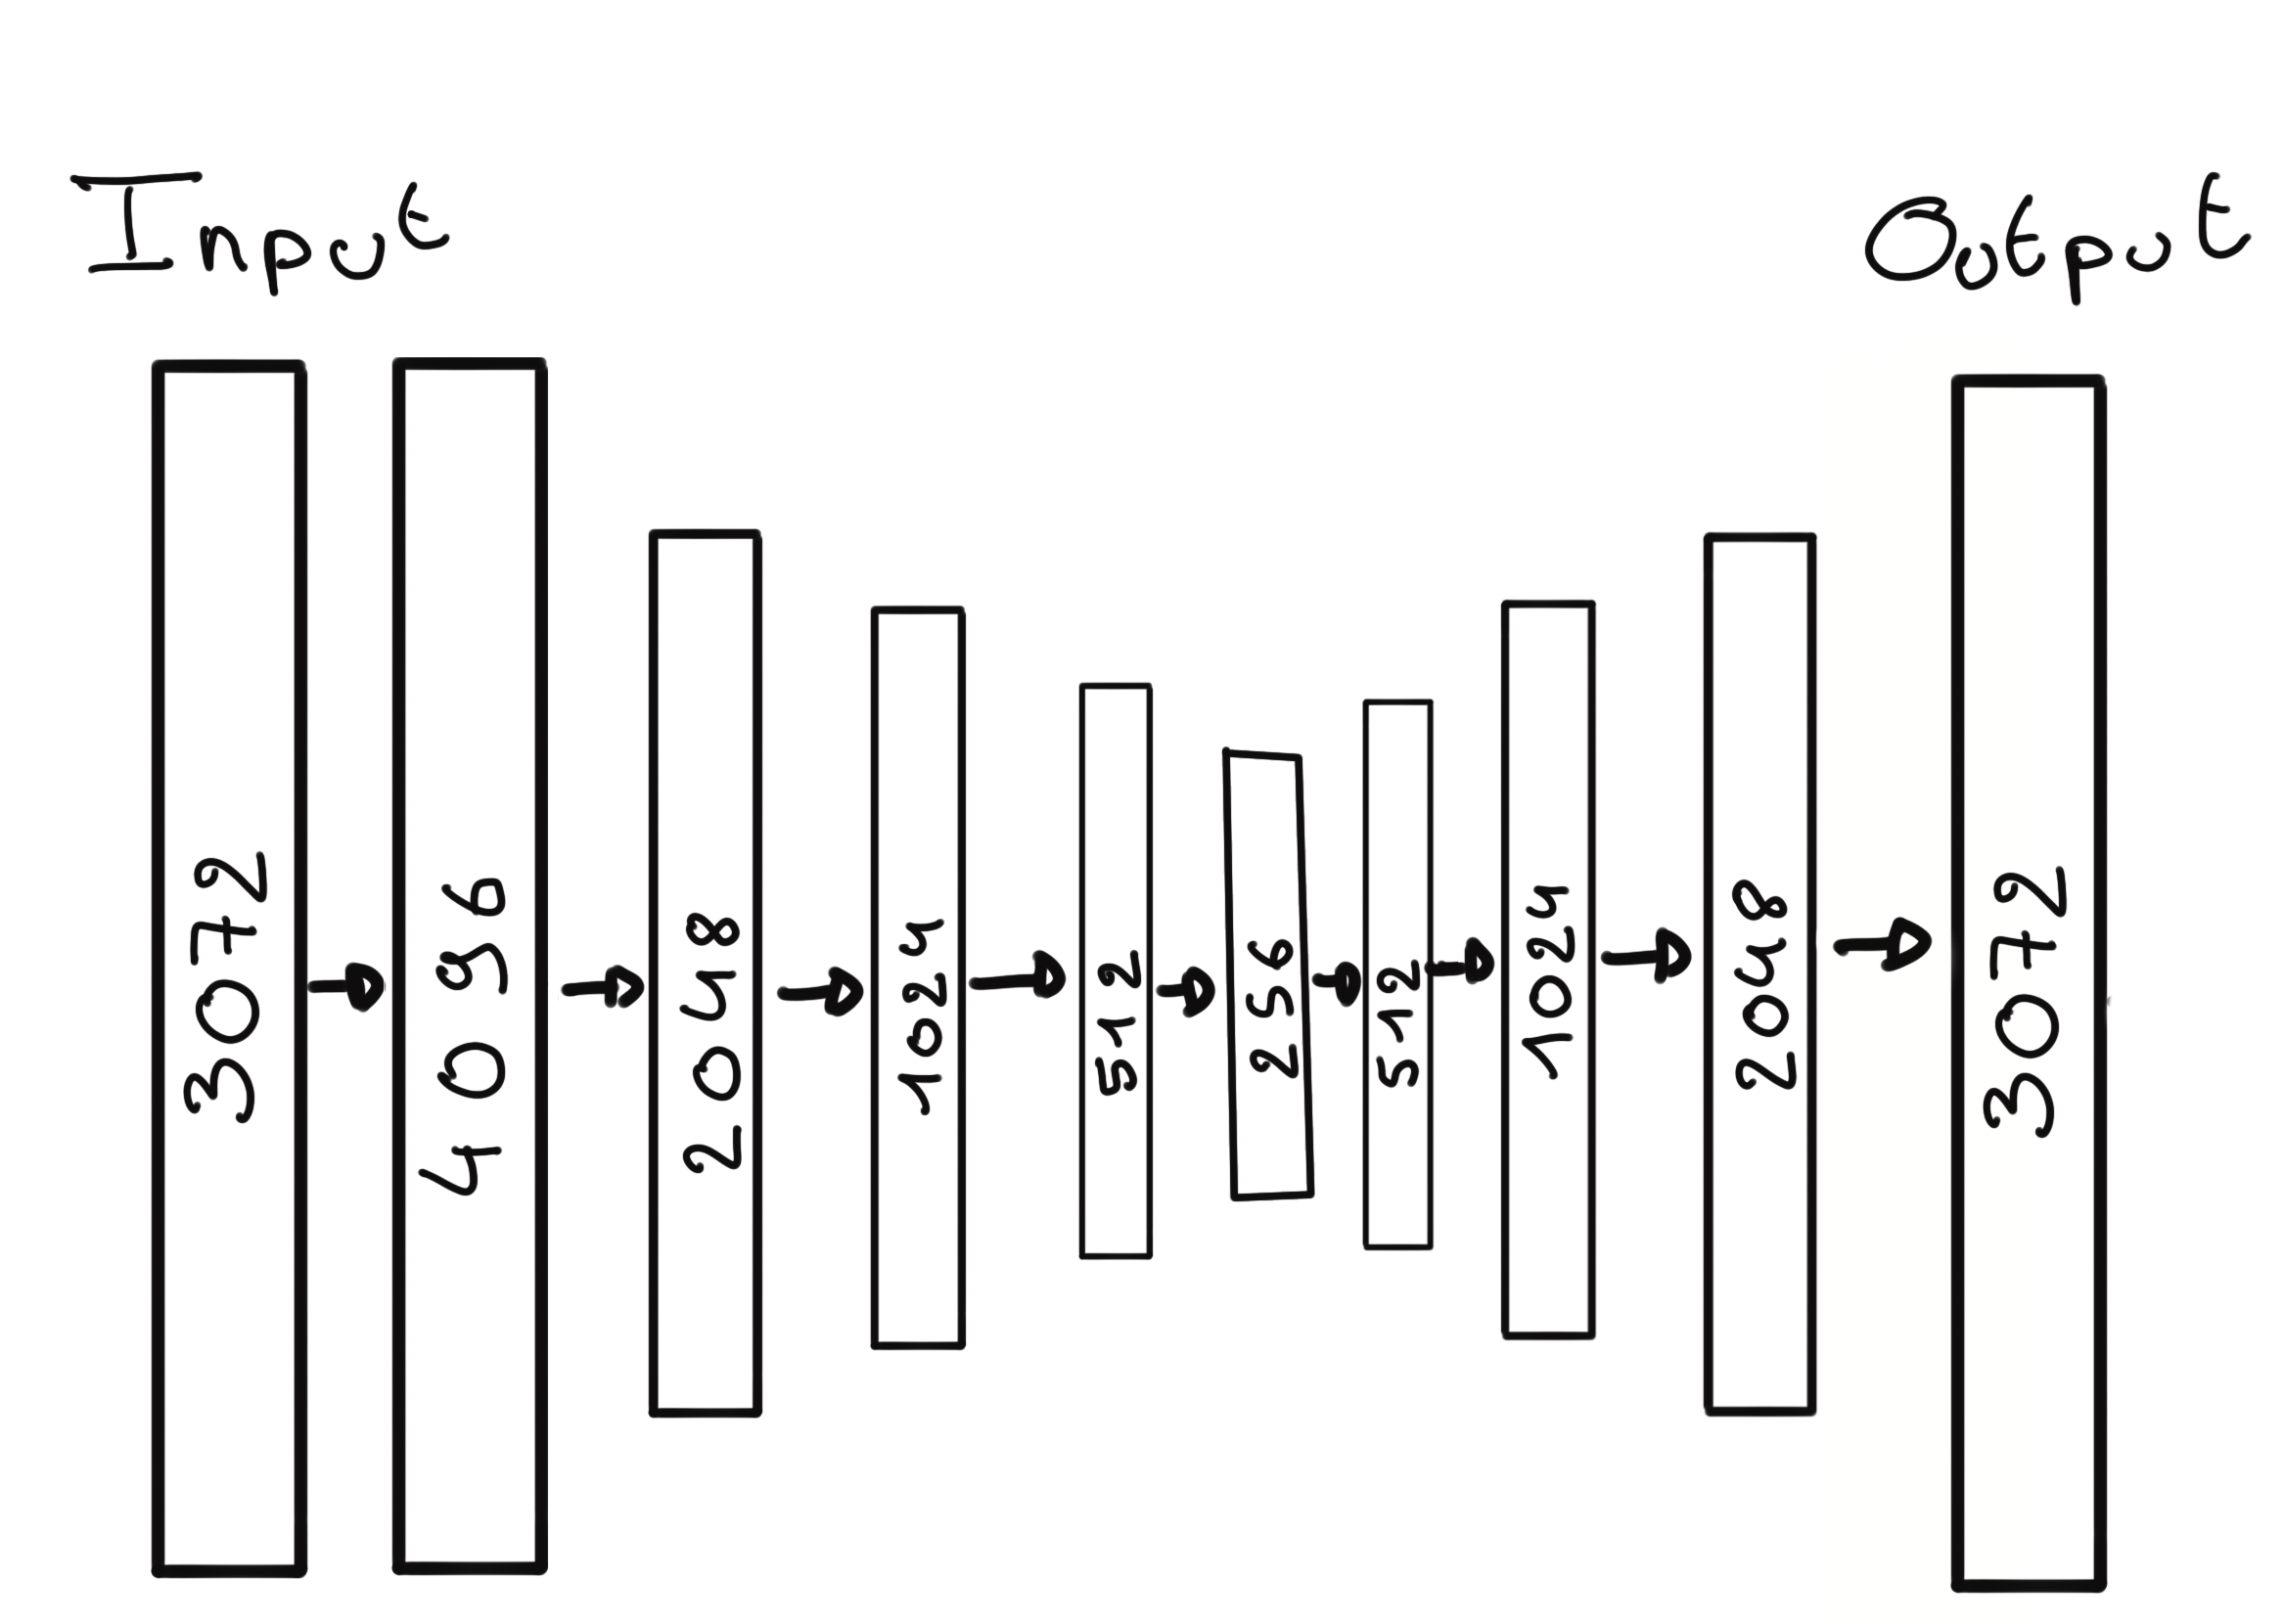
\includegraphics[height=6cm]{images/janne/ANN_illustration.png}
  \caption{Illustration of the ``bottleneck'' architecture of the ANN. Each block represent a fully connected layer with, on the left, the input layer and on the right the output layer. We see a first reduction of the number of neurons per layer, going from 4096 to 256, followed by an augmentation back to 4096 neurons, thus the ``bottleneck''}
  \label{fig:janne:ann_arch}
\end{figure}

The idea behind this architecture is that, by reducing the number of neurons per layer, we force the network to summarize the event in 256 parameters, that it will use to regenerate an event. This architecture has also the advantage of keeping the number of learnable parameters relatively small, as the connection between small layers do not require a lot of parameters.

\subsubsection{ANN loss}

As it was mentioned in the introduction of Section \ref{sec:janne:arch}, the loss of the ANN is composed of two losses, the adversarial loss ${\cal L}_{adv}$ and the regularisation loss ${\cal L}_{reg}$. To those two losses, we adjoin a penalty term that prevent the ANN from producing non-physical events.
\begin{equation*}
  {\cal L} = {\cal L}_{adv} + {\cal L}_{reg} + P
\end{equation*}

The adversarial loss ${\cal L}_{adv}$ is defined as the absolute value correlation between the reconstructed energy and the energy deposit (Eq. \ref{eq:janne:ladv}). The regularisation loss ${\cal L}_{reg}$ is the MSE of the true and reconstructed energy position vector $(x, y, z, E)$ (Eq. \ref{eq:janne:lreg}).


The penalty term is here to prevent the network from generating event that are too far from the initial event. The penalty $P$ is a function that takes the pixelated event $X$, its transformation after the ANN ${\cal G}(X)$ and a constraint $\epsilon$
\begin{equation}
  P(X, {\cal G}(X), \epsilon) = \sum_{i=1}^{3072} \left( ReLU(-{\cal G}(X)_i) + D_i \right)
\end{equation}
with
\begin{equation}
  D_i = \begin{cases}
    \frac{(X_i - {\cal G}(X)_i)^2}{X_i^2}& \text{if } \frac{|X_i - {\cal G}(X)_i|}{X_i} > \epsilon \\
    0& \text{otherwise}
  \end{cases}
\end{equation}
where $i$ index the Healpix pixels. The term $ReLU(-{\cal G}(X)_i$ is minimal, equal 0, when the charge after perturbation is positive. This term prevent the ANN from producing negative charge, feat impossible for the PMTs. The second term $D_i$ is equal 0 when the relative charge between the original and perturbed pixel is less than $\epsilon$. Otherwise, it is the square of this relative charge difference. This term penalize the ANN from producing charges too different from the original event.
\hfill

When dealing with multiple losses like this, it is important tot compare them, as we do not want one term to absorb the other.

The loss ${\cal L}_{adv}$ range from 0 to 1 while ${\cal L}_{reg}$ is 0 when the vertex is perfectly reconstructed by it can theoretically go up to infinity. In practice we expect it to take value of the order of magnitude coherent with the reconstruction performances. In fact, if it would take higher value, it would mean that the reconstruction would reconstruct the event far away from the true vertex in comparison to the expected performance. This kind of issue would be immediately be detected, even with simplistic reconstructions such as the charge barycenter, which goes against the goal of producing subtle fluctuation.

We evaluate ${\cal L}_{reg}$ with $(x, y, z)$ in meter and $E$ in MeV. If the event is reconstructed with a precision of 15 cm and an energy resolution of 3\% at 1 MeV, here taking the reconstruction performance of the best reconstruction algorithm OMILREC (see Sections \ref{sec:juno:reco} and \ref{sec:jgnn:results}), ${\cal L}_{reg} \approx 0.3^2 + 0.03^2 = 0.0909$. We see about an order of magnitude between ${\cal L}_{adv}$ and ${\cal L}_{reg}$. To compensate for it we weight ${\cal L}_{reg}$
\begin{equation}
  {\cal L} = {\cal L}_{adv} + 60\cdot{\cal L}_{reg} + P(\epsilon)
\end{equation}

The amplitude of $P$ and the value of $\epsilon$ will be further discussed in Section \ref{sec:janne:arch:training}.

\subsubsection{Hyperparameter optimization}
%\label{sec:janne:arch:hyper}
%\begin{itemize}
%  \item Pour les meme raison que l'ANN:
%    \begin{itemize}
%      \item Phase exploratoire, architecture tres changeante, random search n'est pas viable
%      \item Architecture consomme beaucoup, besoin d'entrainer sur l'A100
%      \item Possiblement que de l'optimization permetterais de faire passer sur V100, mais developement techniques necessaires.
%    \end{itemize}
%\end{itemize}

All the ANN hyperparameters presented above have been optimized through the numerous iteration the architecture went through. The training is computationally expensive as we need to host both of the network on the GPU card, reaching quickly the memory limit of the GPU. The training of the ANN can takes up to 90h. The requirement of having a powerful GPU can be met locally, as Subatech possess an available A100 \cite{noauthor_nvidia_nodate-1} card with 40GB of memory but we could not port over computing center as they only possess V100 \cite{noauthor_nvidia_nodate-2} GPU with 20GB of memory.

Those constraint made a random search optimization impossible. It is maybe possible, through optimisation, to reduce the memory requirements to reach the threshold to run on V100 but the challenge was deemed not worth it for an exploratory work.

\section{Training of the ANN}
\label{sec:janne:arch:training}
%\begin{itemize}
%  \item Presentation du dataset
%  \item 2 etapes d'entrainement
%  \item Retour à l'identitié -> que l'ANN ne fasse pas n'importe quoi
%  \item Cassage de la reconstruction
%\end{itemize}

The training of the ANN goes through two phases. The first one consist on producing physical events, the second one into searching for perturbations. For both phases, we use the both of the datasets presented in section \ref{sec:janne:method}. We use a batch size of 64 for both datasets meaning that, for each steps, the network see 128 events.

Each epochs goes through the entirety of the training dataset.

\subsection{First training phase: back to physics}
\label{sec:janne:results:identity}

When the ANN is created, before any training has been done, its parameters are initialized with random value. Multiple initialization methods exist. In this work, we go with a common He initialization \cite{he_delving_2015}, which is the default initialization in the PyTorch \cite{ansel_pytorch_2024} library. If we were to ask for an event from the ANN without training first, the results would be random noise. We thus first have it to learn to produce physically sound events.

For this we go for a training of 200 epochs where the loss consist only of the penalty loss. For scaling purpose , the penalty $P$ is scaled by 0.25.
\begin{equation}
  {\cal L}_1 = 0.25 \cdot P(\epsilon = 0.01)
\end{equation}
During this phase, the only objective of the network is to yield events that are the same as the original event.

The evolution of this loss ${\cal L}_1$ during the training for the training dataset and the validation dataset is presented in Figure \ref{fig:jann:train:phase_1}.
\begin{figure}[ht]
  \centering
  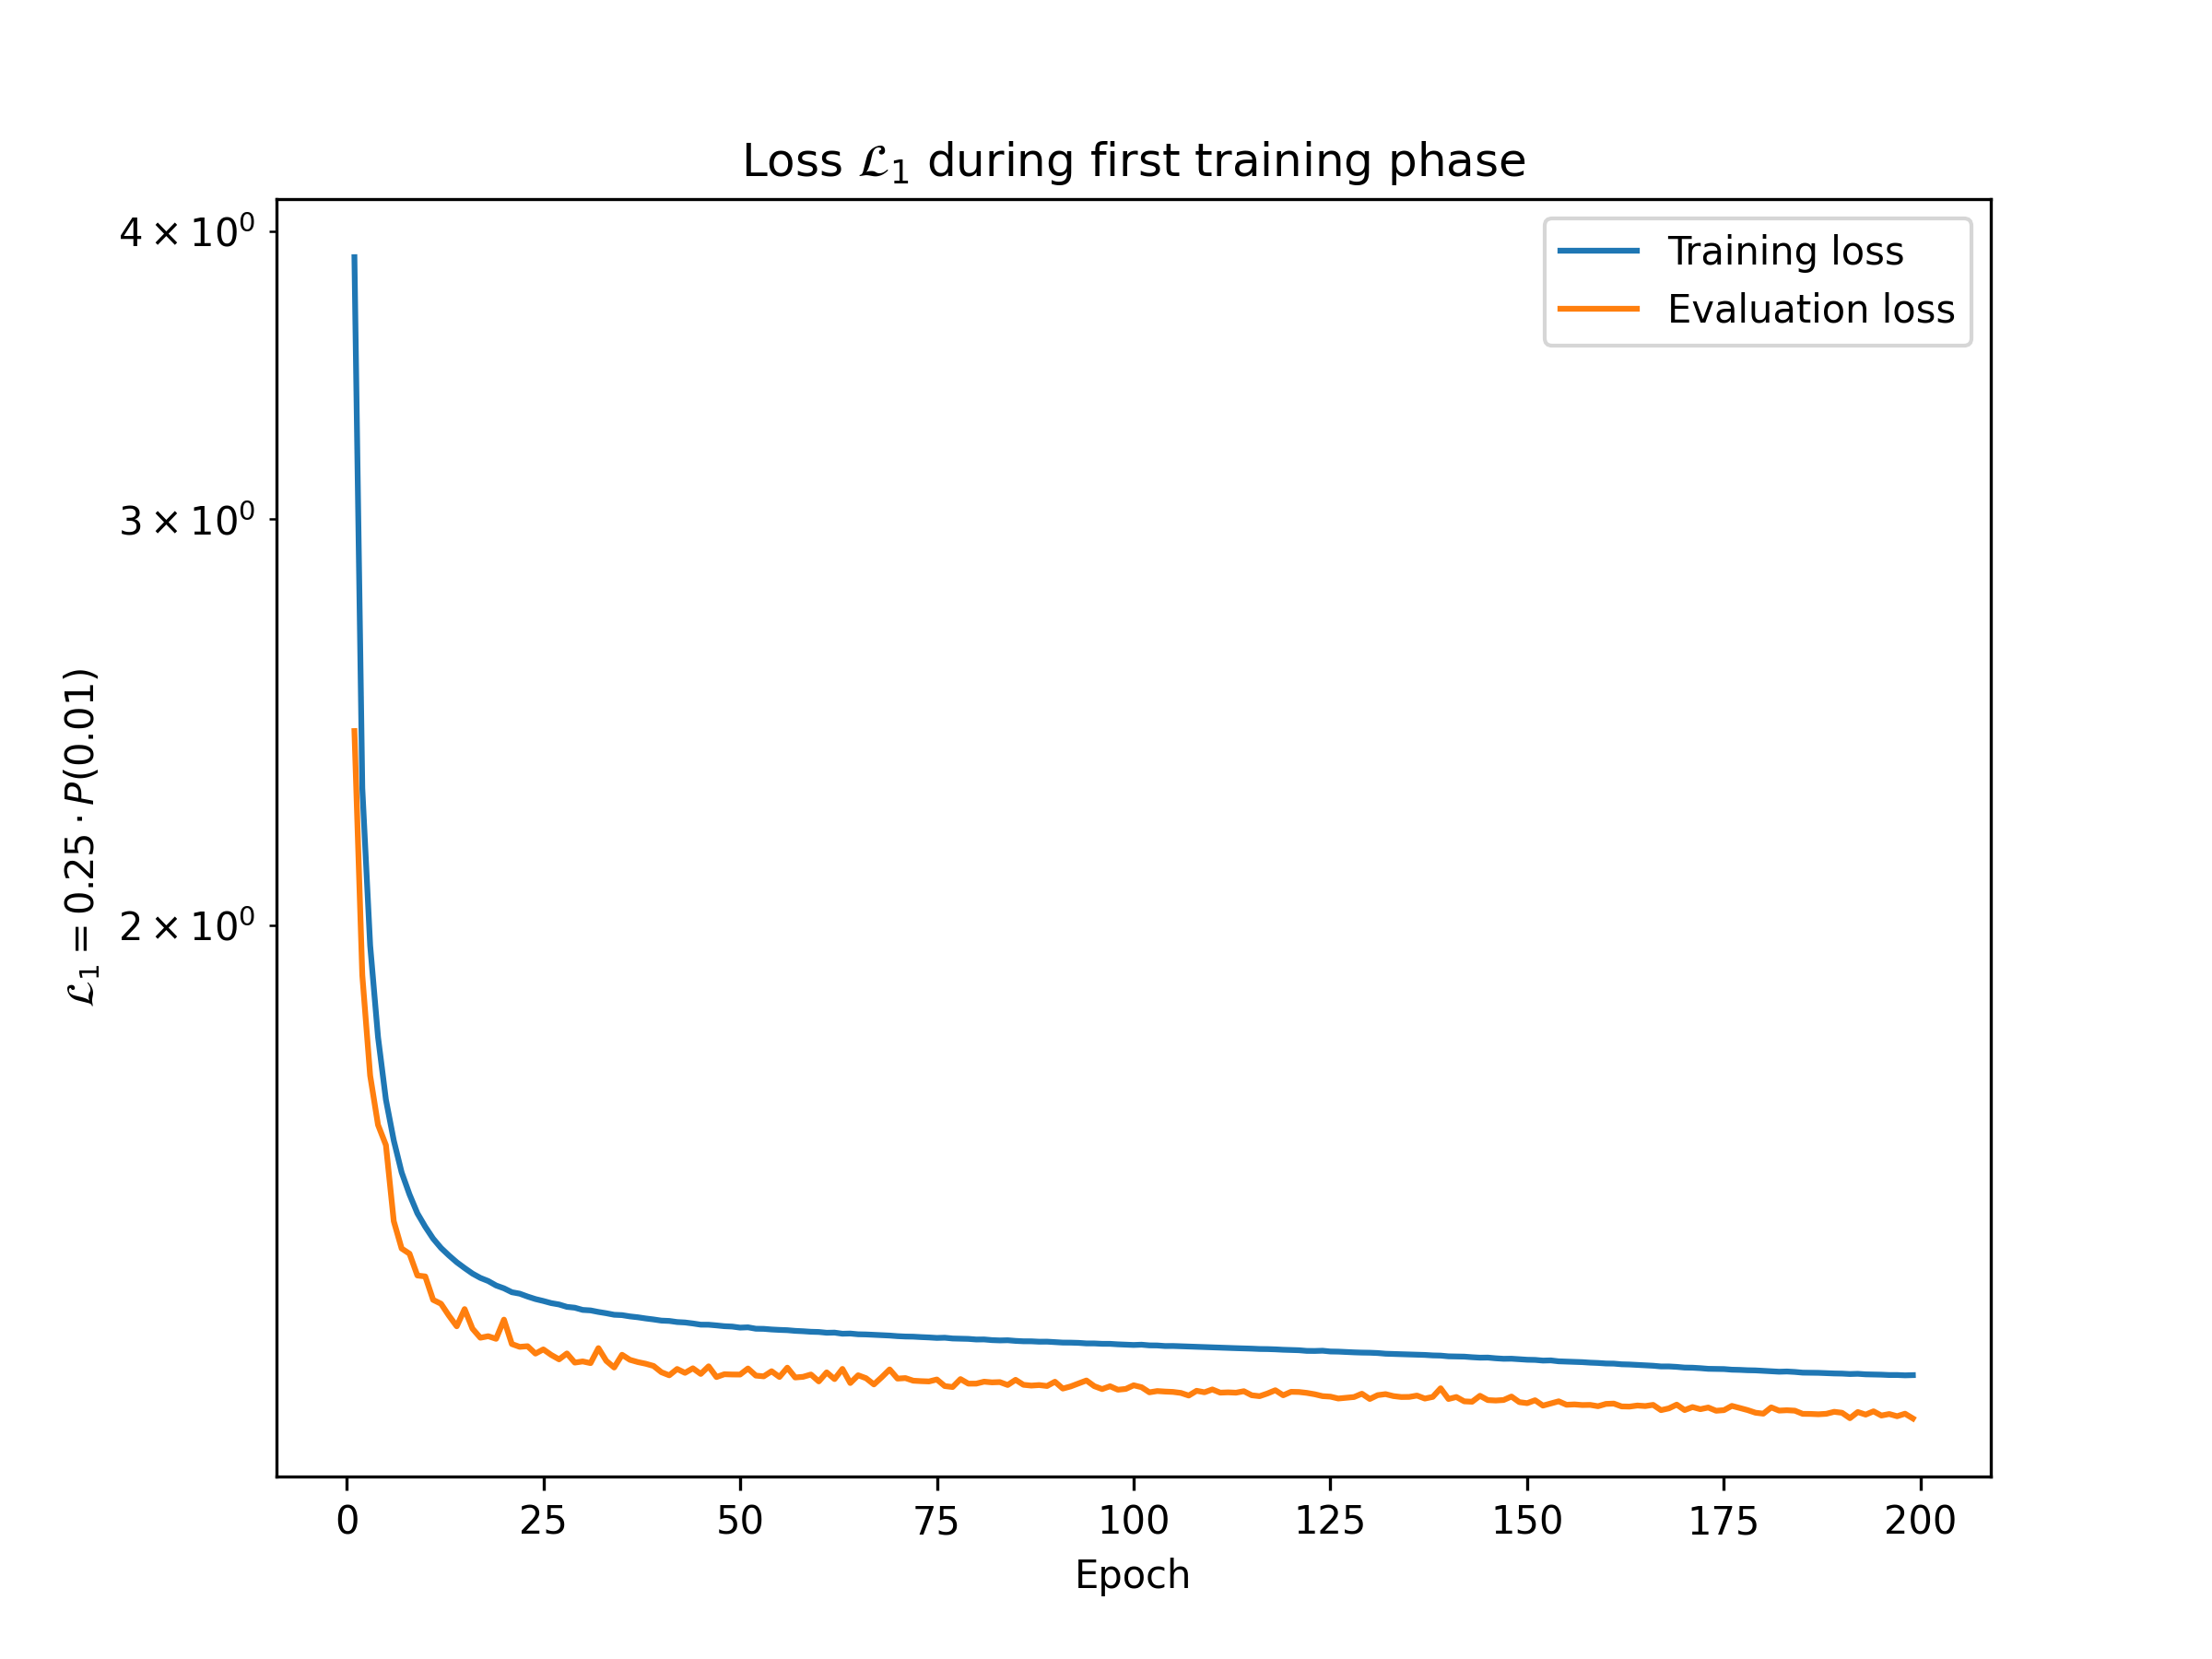
\includegraphics[height=6cm]{images/janne/training/phase_1_penal.png}
  \caption{Evolution of the loss ${\cal L}_1 = 0.25 \cdot P(0.01)$ during the first phase of the training}
  \label{fig:jann:train:phase_1}
\end{figure}
We see that the ANN converge to some stability in the loss.

The time and charge channels of two events after this training phase are presented in Figures \ref{fig:janne:hr_he_200} and \ref{fig:janne:lr_le_200}. We remind that the ANN only act on  the charge channel of the event.
\begin{figure}[ht]
  \centering
  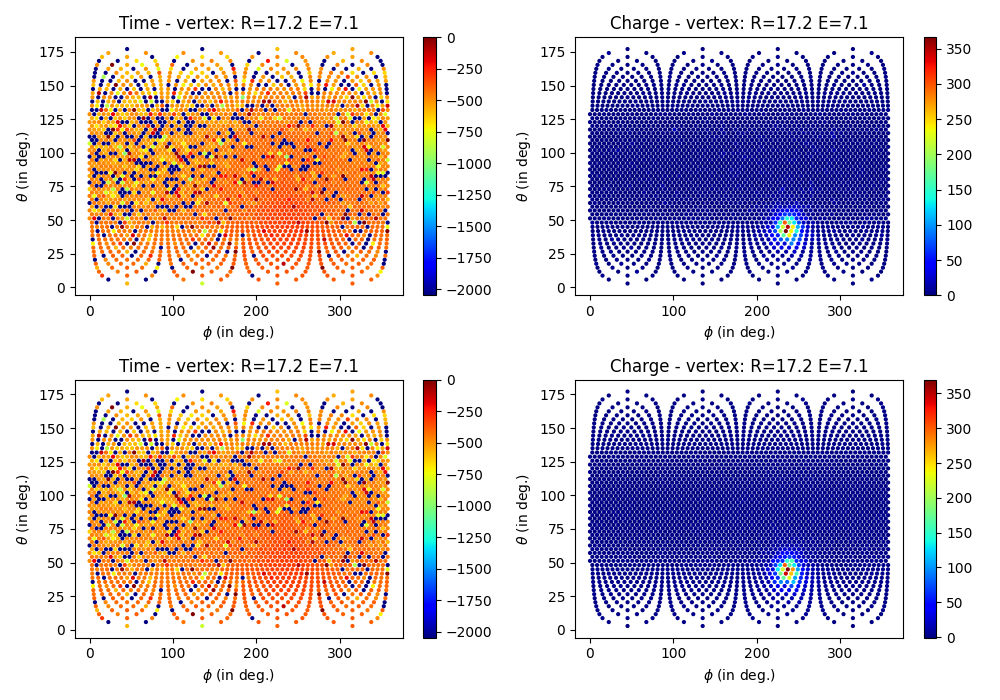
\includegraphics[height=7cm]{images/janne/events/hr_he_200.png}
  \caption{Time channel (on the left) and charge channel (on the right) of a \textbf{radial, high energy event} ($R$ = 17.2 m, $E_{dep}$ = 7.1 MeV), \textbf{Top:} before the ANN perturbation, \textbf{Bottom:} after the ANN perturbation. The ANN have been trained for 200 epochs, just after Phase 1. Time channel in ns and charge channel in $N_{pe}$.}
  \label{fig:janne:hr_he_200}
\end{figure}

\begin{figure}[ht]
  \centering
  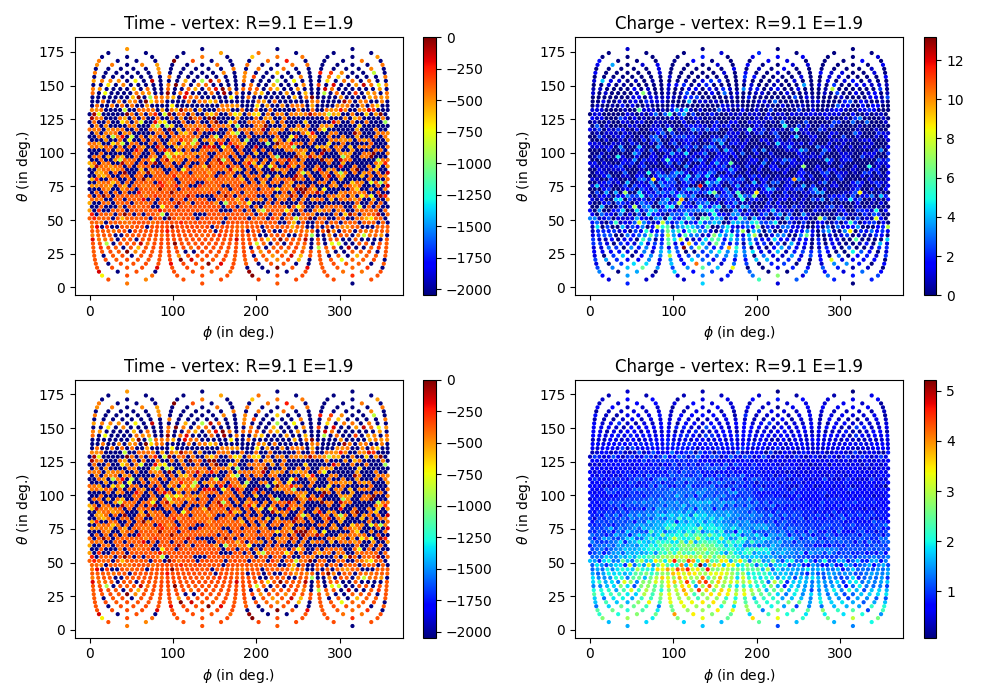
\includegraphics[height=7cm]{images/janne/events/lr_le_200.png}
  \caption{Time channel (on the left) and charge channel (on the right) of a \textbf{central, low energy event} ($R$ = 9.1 m, $E_{dep}$ = 1.9 MeV), \textbf{Top:} before the ANN perturbation, \textbf{Bottom:} after the ANN perturbation. The ANN have been trained for 200 epochs, just after Phase 1. Time channel in ns and charge channel in $N_{pe}$.}
  \label{fig:janne:lr_le_200}
\end{figure}

We observe that for a localized event, Figure \ref{fig:janne:hr_he_200}, the ANN reproduce correctly the event while for more a diffuse event, Figure \ref{fig:janne:lr_le_200}, it produce more ``uniform'' charge distribution. By looking at the color scale in Figure \ref{fig:janne:lr_le_200}, we observe that the ANN do not reproduce singular high number of $N_{pe}$. The highest pixel in the original was 12 $N_{pe}$ whereas, after the ANN, the highest pixel is 5 $N_{pe}$. Furthermore, where in the original event the charge repartition, while diffuse, was still concentrated in specific pixel, the ANN spread the charges in every the pixels.

\subsection{Second training phase: Breaking of the reconstruction}
\label{sec:janne:results:break}

Once the ANN is able to reproduce physical events, we change the loss so it start to search for potential perturbations. For this we introduce the term ${\cal L}_{adv}$ and ${\cal L}_{red}$ producing a second loss ${\cal L}_2$. Adding those terms will significantly change the loss. The previous minima in the parameters phase space the ANN found minimizing ${\cal L}_1$ will not be the minima ${\cal L}_2$. To prevent a gradient explosion, we introduce a growing factor $\lambda$ in front of the term ${\cal L}_{adv}$ and ${\cal L}_{red}$. This factor start at $\lambda  = 0.01$ at epoch 201 and grow $\lambda_{i+1} = \lambda_{i} + 0.01$ where $i$ index the epoch. It cap at $\lambda_{max} = 1$ at epoch 300 after what it stop growing.

Also to ease the task of the ANN, we relax the constraint in the penalty term $P$ from $P(0.01)$ to $P(0.15)$.

The expression of the phase 2 loss ${\cal L}_2$ become:
\begin{equation}
  {\cal L}_2 = \lambda \left( {\cal L}_{adv} + 60 \cdot {\cal L}_{reg} \right) + 0.25 \cdot P(0.15)
\end{equation}

This second phase of the training last for 200 more epochs, up to epoch 400.


\section{Results}
\label{sec:janne:results}
\section{Conclusion and prospect}
\label{sec:janne:conclusion}
\begin{itemize}
  \item Not enough
  \item Probably guide the ANN
\end{itemize}
\end{document}
